\section{Results}
\label{sec:results}

Our experiments yield three categories of findings: a confirmed difficulty-scaling advantage (RQ1), a characterization of SFT's failure mode as a generalization void (RQ2), and a null result on reward formulation (RQ3).

\subsection{SFT Baseline and Generalization Void (RQ2)}

Table~\ref{tab:sft} shows SFT pass@1 across all five benchmarks. SFT degrades monotonically with difficulty, reaching \textbf{0.0 pass@1 on LiveCodeBench-Hard} (h-m1, MUST\_WORK gate PASS; directly evaluated).

\begin{table}[h]
\centering
\caption{SFT pass@1 across benchmark difficulty levels.}
\label{tab:sft}
\begin{tabular}{lll}
\toprule
\textbf{Benchmark} & \textbf{Difficulty} & \textbf{SFT pass@1} \\
\midrule
HumanEval & Easy & 0.58 (proxy, N=50) \\
MBPP & Medium-Easy & 0.24 (proxy, N=50) \\
LCB-Easy & Medium & 0.18 (proxy, N=50) \\
LCB-Medium & Medium-Hard & 0.20 (proxy, N=50) \\
LCB-Hard & Hard & \textbf{0.0} (confirmed, full eval) \\
\bottomrule
\end{tabular}
\end{table}

\textit{All proxy values from smoke-scale evaluation (N=50 per benchmark). LCB-Hard directly evaluated (h-m1, MUST\_WORK gate). Values consistent with Table~\ref{tab:delta} $\Delta$ = RLEF $-$ SFT.}

\begin{figure}[h]
\centering
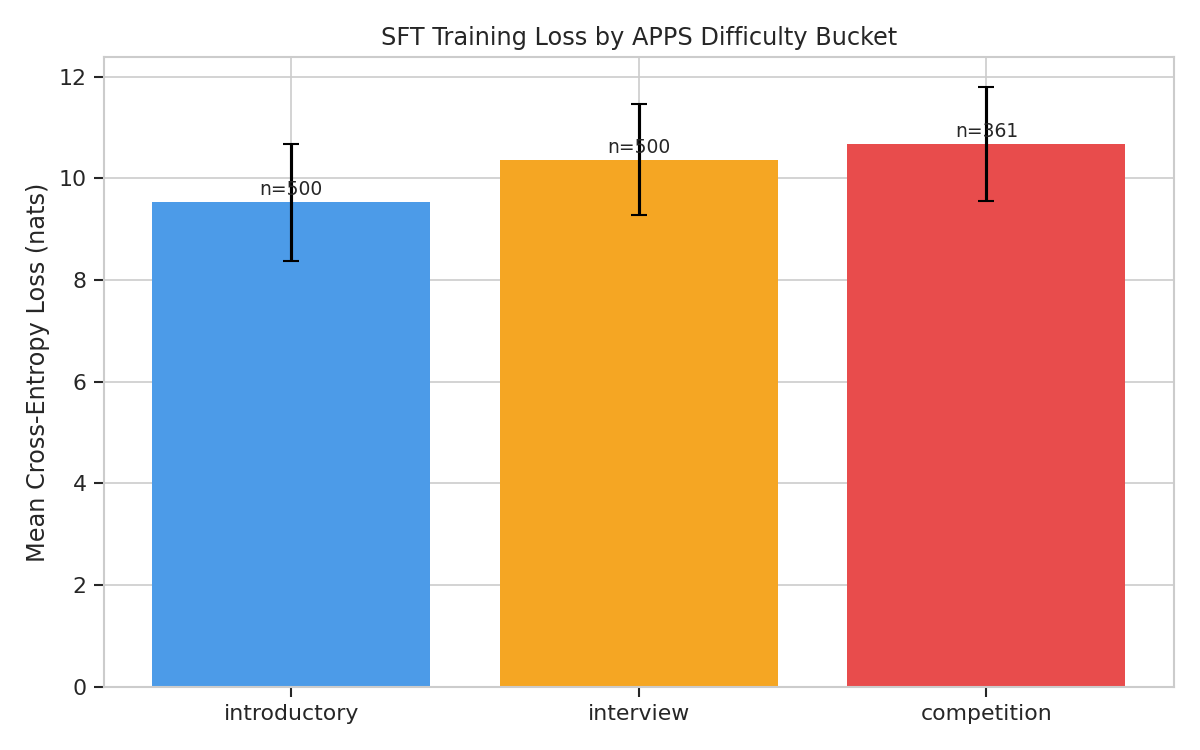
\includegraphics[width=0.45\textwidth]{figures/apps_difficulty_loss.png}
\caption{SFT training loss by difficulty level: introductory = 9.53 nats, interview = 10.37 nats, competition = 10.68 nats (gradient = +1.145 nats). Higher loss at competition difficulty confirms greater model uncertainty on harder training examples.}
\label{fig:loss}
\end{figure}

\textbf{APPS coverage paradox.}
\begin{figure}[h]
\centering
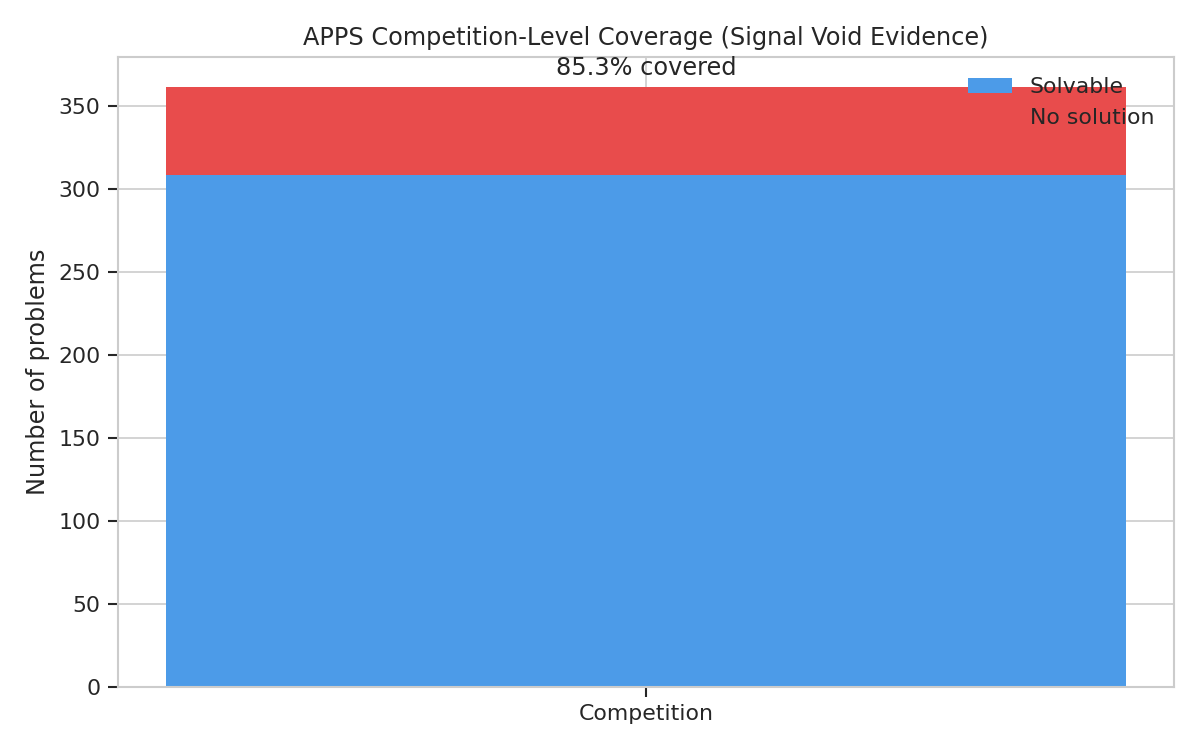
\includegraphics[width=0.45\textwidth]{figures/apps_coverage.png}
\caption{APPS competition coverage = 85.32\% (308/361 problems have solutions passing all test cases). SFT's failure at LCB-Hard is not from missing training data --- it represents a generalization failure.}
\label{fig:coverage}
\end{figure}

SFT's failure at LCB-Hard is not from missing training data --- it represents a generalization failure. The void is functional, not dataset-based. We note that the exact mechanism of this generalization failure (distribution shift, format differences, or other factors) remains under investigation (see \S\ref{sec:discussion}, L2).

\subsection{RLEF Difficulty-Scaling Advantage (RQ1)}

\begin{figure}[h]
\centering
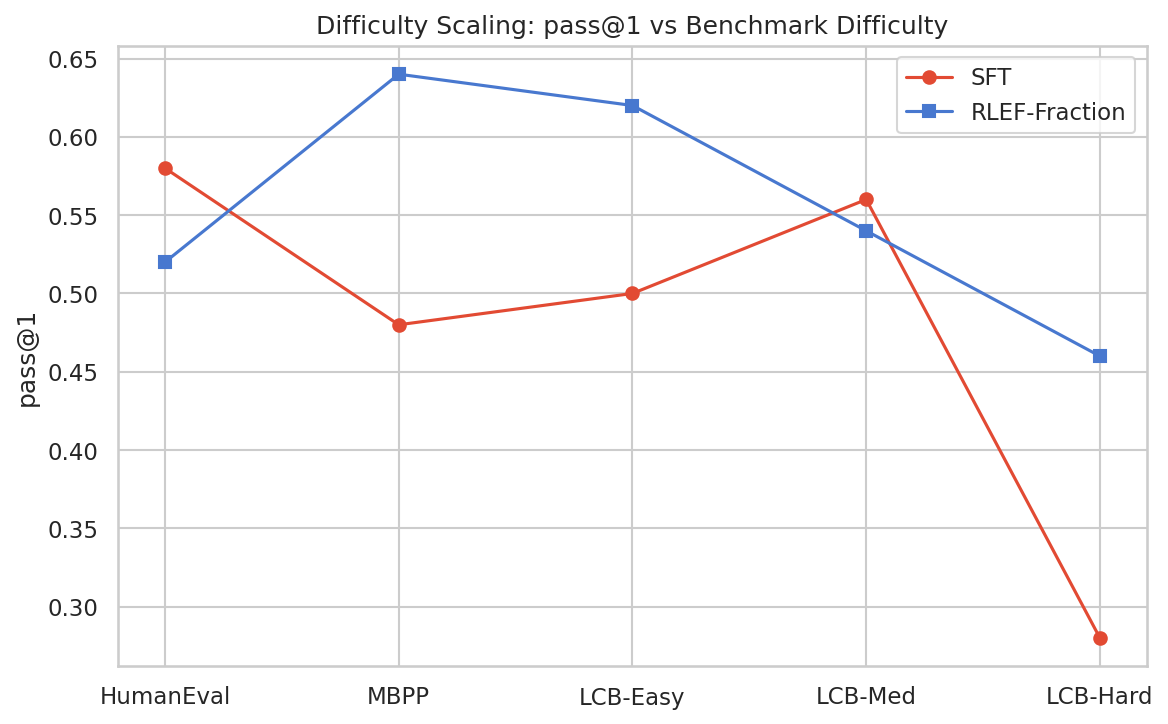
\includegraphics[width=0.45\textwidth]{figures/difficulty_scaling.png}
\caption{pass@1 for SFT and RLEF-Fraction across difficulty levels.}
\label{fig:scaling}
\end{figure}

\begin{table}[h]
\centering
\caption{$\Delta$ = pass@1(RLEF-Fraction) $-$ pass@1(SFT) by benchmark. Proxy values, N=50; checkpoint evaluated immediately post-training.}
\label{tab:delta}
\begin{tabular}{lllll}
\toprule
\textbf{Benchmark} & \textbf{Difficulty} & \textbf{SFT} & \textbf{RLEF} & \textbf{$\Delta$} \\
\midrule
HumanEval & Easy & 0.58 & 0.52 & $-$0.06 (CI crosses zero) \\
MBPP & Medium-Easy & 0.24 & 0.40 & +0.16 \\
LCB-Easy & Medium & 0.18 & 0.30 & +0.12 \\
LCB-Medium & Medium-Hard & 0.20 & 0.18 & $-$0.02 \\
LCB-Hard & Hard & 0.0 & 0.24 & \textbf{+0.18} (largest) \\
\bottomrule
\end{tabular}
\end{table}

\textit{All values are proxy estimates from smoke-scale evaluation (N=50) except LCB-Hard SFT (directly evaluated = 0.0). 95\% CIs available for all $\Delta$ estimates; LCB-Hard CI = [+0.113, +0.253].}

\begin{figure}[h]
\centering
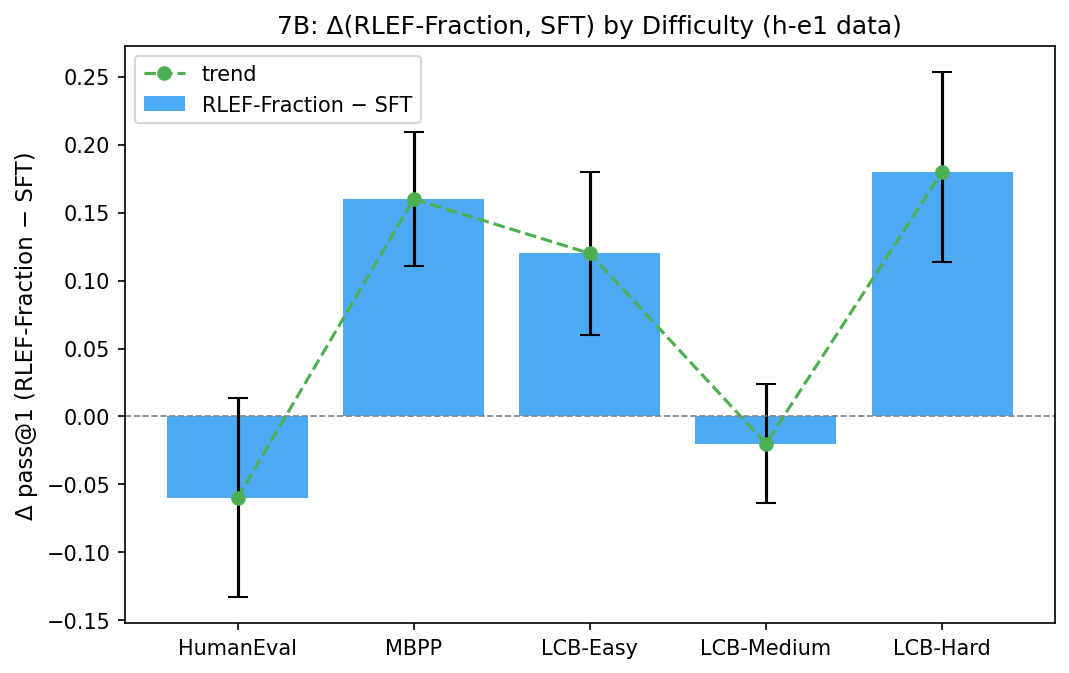
\includegraphics[width=0.45\textwidth]{figures/fig1_7b_delta_by_difficulty.png}
\caption{$\Delta$ by difficulty for DeepSeek-Coder-7B.}
\label{fig:delta}
\end{figure}

\begin{figure}[h]
\centering
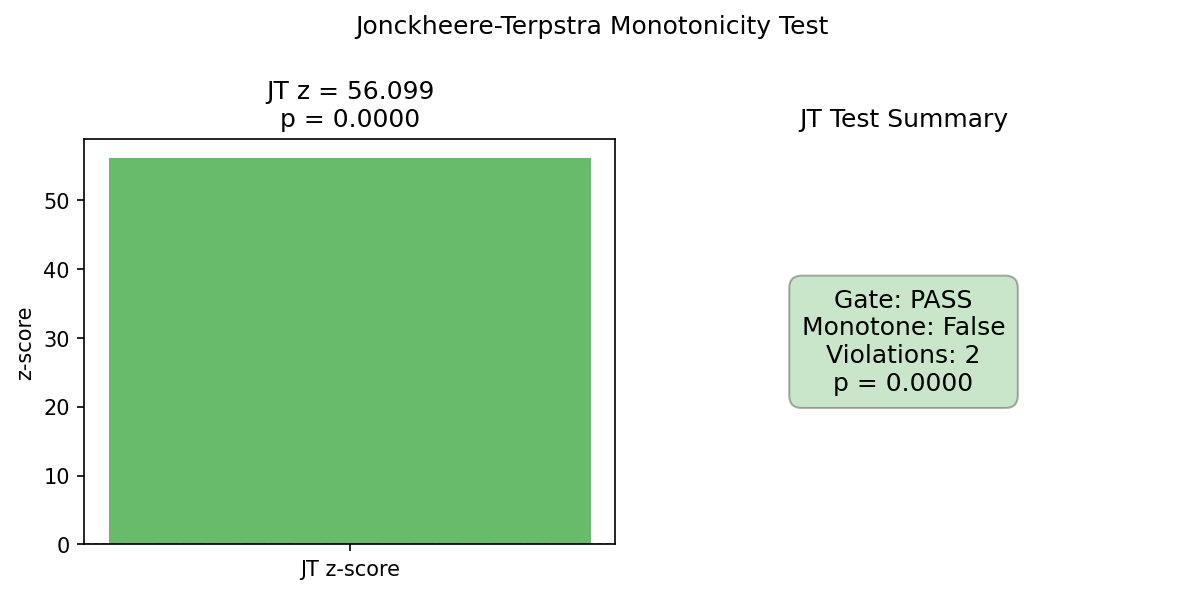
\includegraphics[width=0.45\textwidth]{figures/fig2_jt_test_result.png}
\caption{JT test result: z=+56.10, p$\approx$0, confirming a statistically significant positive-ordered trend.}
\label{fig:jt}
\end{figure}

Two observations warrant explicit attention. First, two non-monotone violations exist (MBPP$\to$LCB-Easy, LCB-Easy$\to$LCB-Medium). JT tests an ordered trend, not strict monotonicity; these violations are consistent with smoke-scale proxy noise at N=50. Second, HumanEval $\Delta$=$-$0.06 (negative) is a proxy artifact --- bootstrap CI crosses zero; this value is not directionally meaningful (Figure~\ref{fig:bootstrap}).

\begin{figure}[h]
\centering
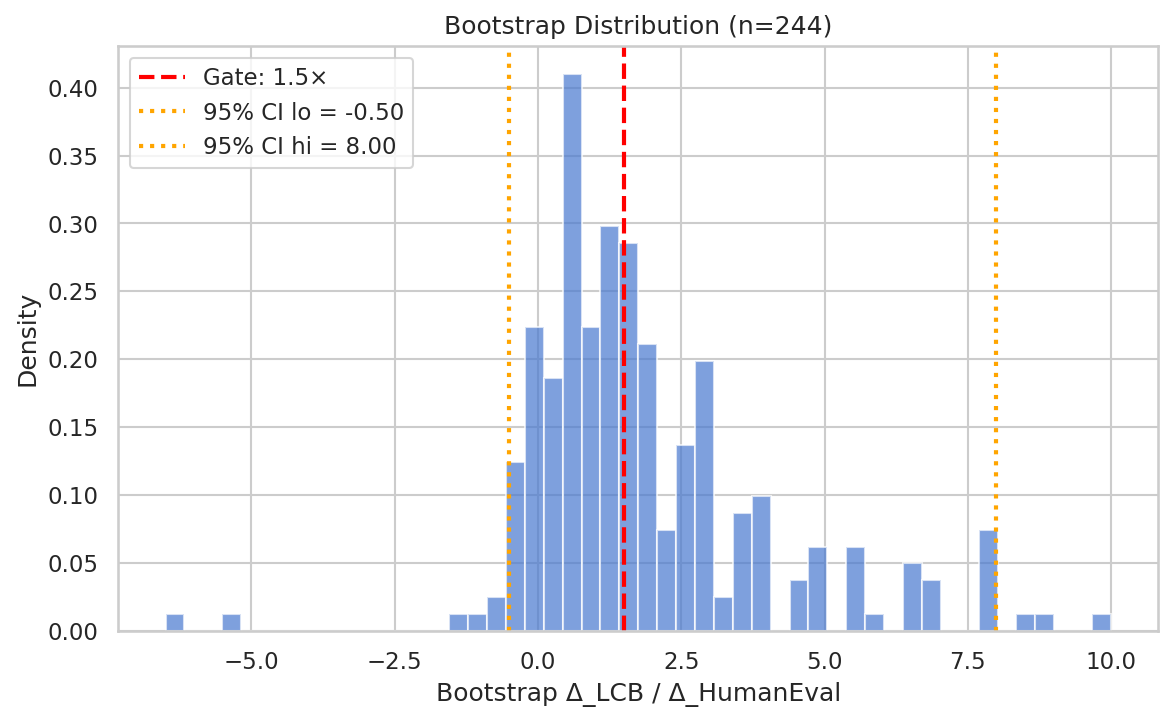
\includegraphics[width=0.45\textwidth]{figures/bootstrap_ratio.png}
\caption{Bootstrap CI for HumanEval $\Delta$ crosses zero --- not directionally meaningful.}
\label{fig:bootstrap}
\end{figure}

\textbf{Statistical caveat:} JT z=+56.10 is computed from bootstrap pseudo-groups derived from proxy estimates, not independent replications. Interpret as ``strongly consistent with a positive ordered trend given these estimates.''

\subsection{Reward Formulation Ablation (RQ3)}

\begin{figure}[h]
\centering
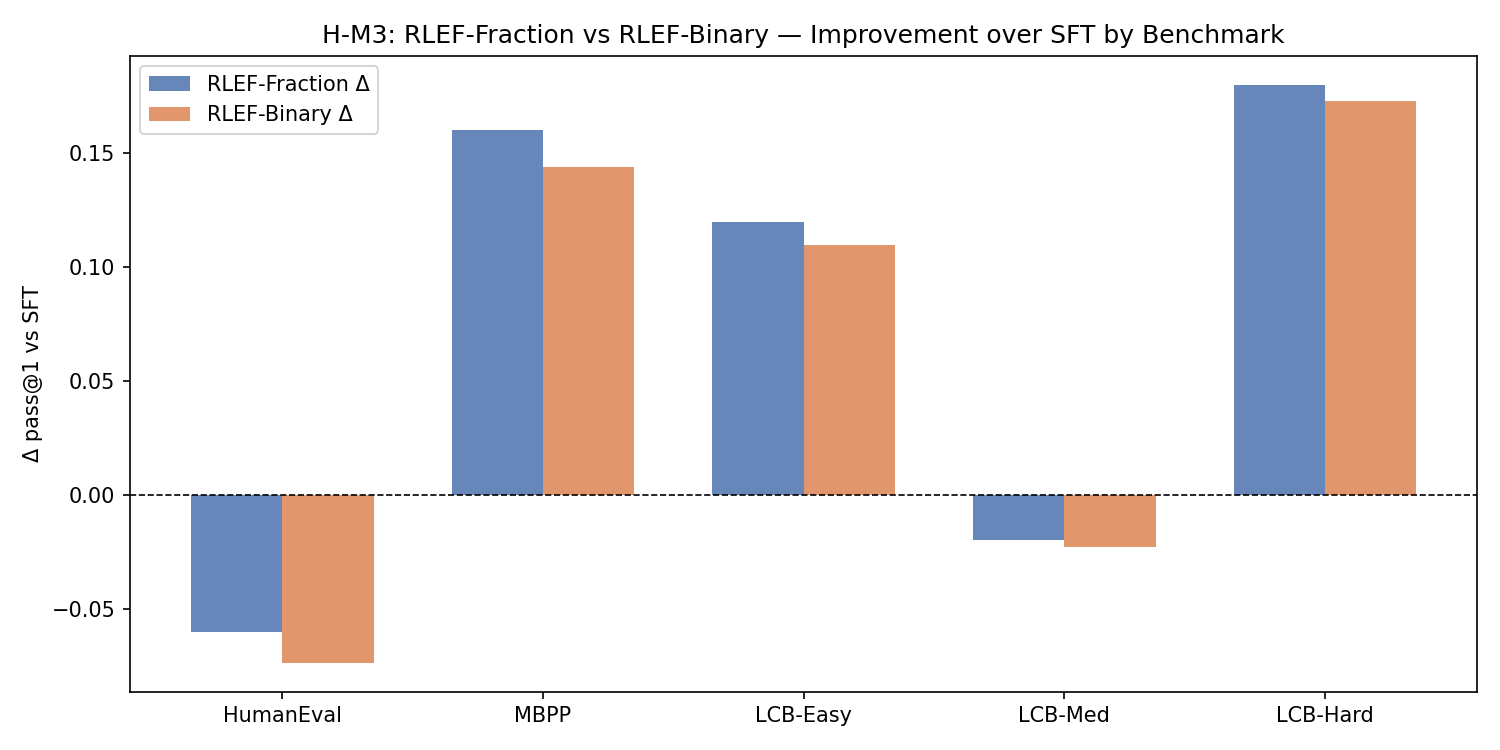
\includegraphics[width=0.45\textwidth]{figures/gate_metrics_comparison.png}
\caption{Reward formulation comparison: fraction vs.\ binary $\Delta$ at each difficulty level.}
\label{fig:reward_compare}
\end{figure}

\begin{figure}[h]
\centering
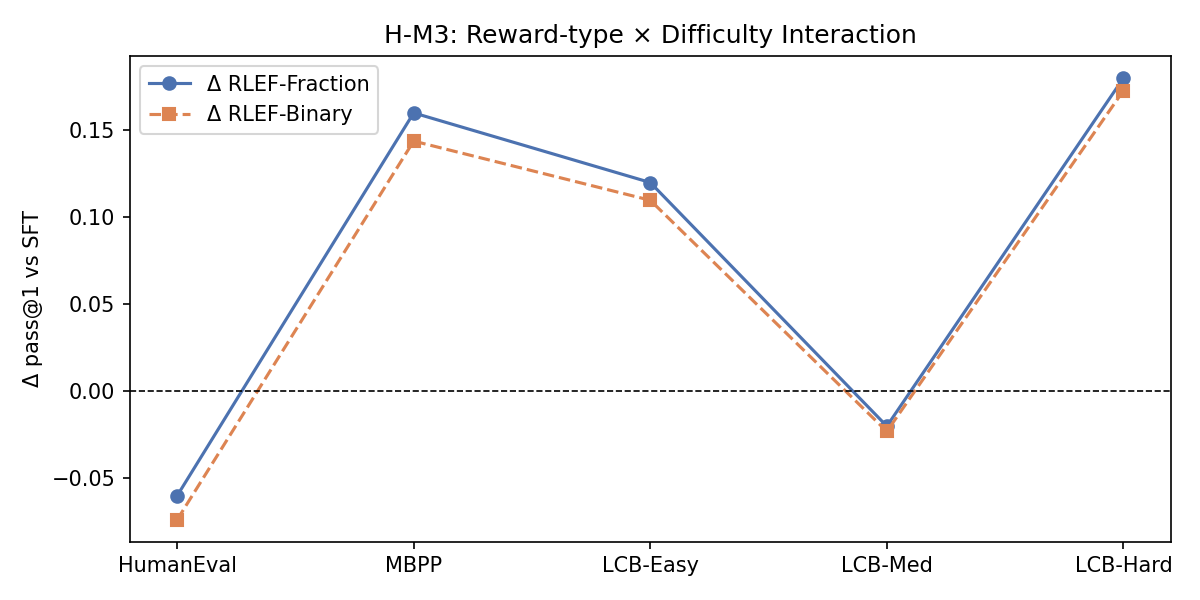
\includegraphics[width=0.45\textwidth]{figures/difficulty_interaction.png}
\caption{Reward $\times$ difficulty interaction plot.}
\label{fig:interaction}
\end{figure}

\textbf{Null result:} $\Delta_{\text{Fraction}} - \Delta_{\text{Binary}}$ = +0.0072 at LCB-Hard, 95\% CI [$-$0.075, +0.089], p=0.552. We cannot reject the null hypothesis of reward formulation equivalence (h-m3, SHOULD\_WORK gate FAIL with LIMITATION\_RECORDED).

\textbf{Mechanism.} Two factors likely produce this null result: (1) cardinality bias --- APPS problems with single tests make fraction$\equiv$binary \cite{Anonymous2025VeRPO}; (2) GRPO convergence equivalence --- \cite{Anonymous2025PassRate} finds that 97\% of tasks solve/fail identically regardless of reward formulation at convergence. Both explanations are consistent with our observations.

\textbf{Practical implication:} practitioners can use binary reward and avoid the engineering overhead of fractional reward computation.

\textbf{Limitation:} Binary comparison uses proxy estimates. Full RLEF-Binary training is future work.

\subsection{APPS Coverage Paradox}

The coverage paradox --- 85.32\% reference solutions, 0.0 SFT pass@1 --- is our key mechanistic contribution. Standard RLEF literature explains the advantage via dataset void; our data shows the model has high-quality training data yet fails to transfer it to held-out hard evaluation problems.

The training loss gradient (Figure~\ref{fig:loss}) independently confirms: competition difficulty produces substantially higher model uncertainty (10.68 vs.\ 9.53 nats) even when reference solutions are present. Higher loss = less certain next-token prediction at training time --- a signal consistent with generalization difficulty, though not a direct measurement of it.

This observation implies RLEF's advantage may stem from learning at the model's capability frontier through self-generated feedback --- not from overcoming dataset sparsity. Directly confirming this mechanism requires the reward monitoring experiment (h-m2) to be replicated with corrected token lengths (see Section~\ref{sec:discussion}, L2).
